\chapter{\label{chapter4}Evaluation}

In this chapter I will evaluate the convergence time of the iSDX without and with Swift.

\section{\label{chapter4:Test Setup}Test Setup}

\begin{figure}[h]
\center
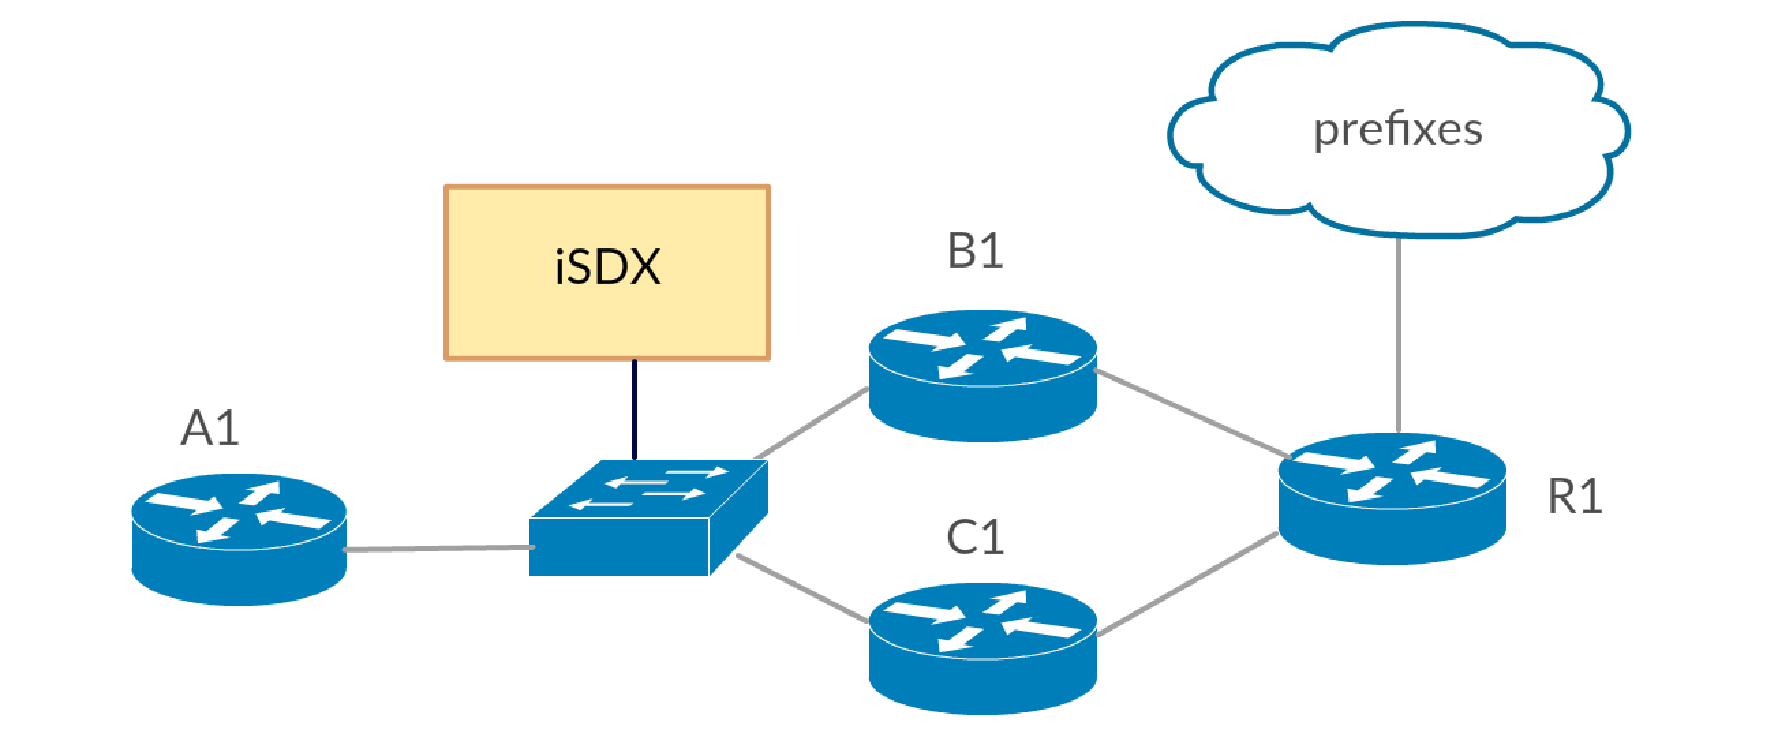
\includegraphics[scale = 0.36]{Figures/eval_exp_setup.pdf}
\caption{Experiment Setup}
\end{figure}

\rb{describe server: 1x4 Cores Xeon CPU E5620 @ 2.40GHz, 36G RAM, linux version, used software: mininet, bgpsimple to inject routes, quagga routers}

The test setup has an iSDX with or without Swift connected to three participants. Participants B1 and C1 are connected to the rest of the internet via R1 and advertise up to 500000 prefixes to A1. Participant A1 prefers routes from B1. Remote failure is simulated by setting the link B1 R1 down. If this link is down A1 needs to updates his RIB, check if flow rules have changed and update the virtual next-hop/vmac for every withdrawn prefix.\\ 
The experiment setup is run in mininet. 



\section{\label{chapter4:Convergence time without Swift}Convergence Time without Swift}

Convergence time is measured as the time between the first withdraw arriving in the route server and the participant controller finishing to process the last withdraw. To measure the convergence time the built in iSDX log server is used.\\
This convergence time does not take into account the hold timer or the time the participant router takes to process the withdrawals. But since these things are not under the control of the iSDX they are ignored in this evaluation.

\begin{figure}[h]
\center
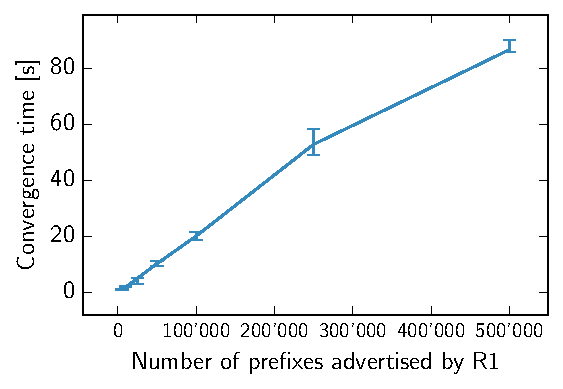
\includegraphics[scale = 1]{Figures/noswift.pdf}
\caption{Convergence time of the iSDX without Swift}
\end{figure}

\newpage

The convergence time increases linearly with the number of prefixes advertised by R1. \\
At 500'000 prefixes the iSDX takes about 90 seconds to converge. During these 90 seconds A1 sends packet to B1, which then get dropped by B1. 

\section{\label{chapter4:Convergence time with Swift}Convergence Time with Swift}

Convergence time is measured as the time between the first withdraw arriving in the route server and the participant controllers FR handler finishing to push the Fast-reroute rules. \\

\begin{figure}[h]
\center
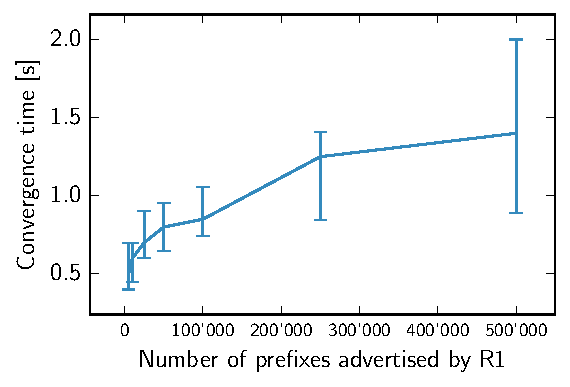
\includegraphics[scale = 1]{Figures/swift.pdf}
\caption{Convergence time of the iSDX without Swift}
\end{figure}

The convergence time increases slightly with higher number of prefixes. At 500'000 prefixes the iSDX takes about 1.5 seconds to push the FR rules. After these 1.5 seconds packets sent from A1 get redirected to C1 and reach their destination. \\
For 500'000 prefixes the convergence time is reduced by a factor of 60.

\newpage